
\newpage
\chapter{Premix laminar flame}

\section{Introduction}
The premix laminar flame model in Camflow is a transient model capable of predicting the species profiles, velocity profiles, and the temperature profile. The model currently simulates a burner-stabilized flame with known mass flow rate. When the temperature profiles are obtained from experiment, the model can be used to simulate only the species profiles by providing the experimentally observed temperature profile. In this case only the species transport equations are solved. An initial guess of intermediate species may be provided to initialize the flow field. If the temperature profile is not known, the model can predict the temperature profile by solving the energy equation. In this case an initial guess for the temperature profile needs to be provided. 

\section{Fundamentals}
The premix laminar flame model solves the equation of continuity
\begin{equation}
 \frac{d (\rho u A_c) }{dz} =0,
\end{equation}
species continuity equation
\begin{equation}
 \rho A_c \frac{\partial Y_k}{\partial t}+ \rho u A_c \frac{\partial Y_k}{\partial z} + \frac{\partial j_k}{\partial z} = A_c\dot{\omega}_k W_k, \quad k=1\ldots K_g
\end{equation}
with $j_k$ defined as
\begin{equation}
 j_k = -\rho D_{km} \frac{dY_k}{dz},
\end{equation}
the energy equation,
\begin{equation}
 \rho c_p \frac{\partial T}{\partial t}+ \rho u c_p \frac{\partial T}{\partial z} - \frac{\partial }{\partial z}\bigg(\lambda \frac{\partial T}{\partial z} \bigg) + \frac{\partial}{\partial z} \sum_k j_k h_{k}  + \sum_k h_k\dot{\omega}_k = 0
\end{equation}
and the equation of state
\begin{equation}
 p\bar{W}=\rho RT.
\end{equation}
In the above equations, $\rho$ is the density in kg/m$^3$, $u$ is the velocity in m/s, $A_c$ is the area of cross section in $m^2$, $Y_k$ is the mass fraction of the k\'th chemical species, $j_k$ the mass flux of the k\'the species in kg/$m^2-s$, $\dot{\omega}_k$ the molar production rate of the k\'the species in mol/m$^3$-s, D$_{km}$ the diffusion coefficient of the k\'the species in the mixture, $h_k$ the specific enthalpy in J/kg, and the $t$ the time in $s$.

\section{Input file}
An example of ``camflow.xml'' input file is shown below
{\scriptsize{

\begin{verbatim}
 
<?xml version="1.0" encoding="ISO-8859-1"?>
<camflow>
   <reactor model="premix">
    <diameter unit="m">0.015</diameter>
    <length unit="m">0.05</length>
  </reactor>
  <op_condition>
     <temperature>adiabatic</temperature>     
    <pressure unit="atm">0.0329</pressure>
  </op_condition>
  <inlet>
     <fuel>
       <velocity unit="m/s">1.0</velocity>
       <temperature unit="K">373.7</temperature>
       <flowrate unit="cgs">4.63e-3</flowrate>
       <molefrac>
        <species name="H2">0.28</species>
        <species name="O2">0.09</species>
        <species name="AR">*</species>
       </molefrac>
     </fuel>
  </inlet>
   <solver mode="segregated" solver="cvode" residual="on">
     <maxTime>10000000</maxTime>
     <iterations>2</iterations>
     <tols>
        <species>
           <aTol>1.e-08</aTol>
           <rTol>1.e-06</rTol>
        </species>
        <temperature>
           <aTol>1.e-03</aTol>
           <rTol>1.e-03</rTol>
        </temperature>
        <flow>
           <aTol>1.e-03</aTol>
           <rTol>1.e-03</rTol>
        </flow>
     </tols>
   </solver>
  <initialize>
    <mCenter unit="cm">1</mCenter>
    <mWidth unit="cm">0.75</mWidth>
    <product name="H2">0.4</product>
    <product name="CO">0.2</product>
    <product name="CO2">0.2</product>
    <product name="CH4">0.2</product>
    <intrmdt name="H">0.1</intrmdt>
    <intrmdt name="OH">0.12</intrmdt>
    <intrmdt name="HO2">0.001</intrmdt>
    <Tprofile unit_L="cm" unit_T="K">
      <position x="0.0">373.7</position>
      <position x="0.125">484.5</position>
      <position x="0.25">583.7</position>
      <position x="0.375">672.2</position>
      <position x="0.5">753.5</position>
      <position x="0.75">901.4</position>
      <position x="1.0">1027.0</position>
      <position x="1.25">1120.0</position>
      <position x="1.5">1184.0</position>
      <position x="2.0">1260.0</position>
      <position x="3.0">1348.0</position>
      <position x="6.0">1475</position>
      <position x="10.0">1524.0</position>
    </Tprofile>
 </initialize>
 <report outfile="final" species="mole">
 </report>
 <grid>grid.inp</grid>
</camflow>
\end{verbatim}}
}


The input file follows xml specification with a number of child elements. Each child element is described in detail below.

\begin{itemize}
 \item \textbf{rector} : The reactor element specifies which model is to be simulated and for a premix laminar flame camflow expects ``premix'' as the model attribute value. The reactor element also holds child element for specifying diameter and the flame height, and each child element is given with the unit attribute. The unit of the value specified can be in ``cm'', ``m'', or in ``in''ches. Appropriate attribute must be specified.

\item \textbf{op\_conditions} : The element op\_conditions describes the operating conditions for the flame. This includes the specification of the pressure and the condition applied to the solution of energy equation. The flame pressure may be specified in the units of ``Pa'', ``atm'', or ``bar''. The temperature element can take the values of ``isothermal'', ``adiabatic'', or ``userdefined''. In the case of isothermal calculation, the energy equation is not solved and the flame is assumed to be at the same temperature as the incoming fuel. The user may also perform the integration for a pre-calculated or measured temperature profile. In this case the temperature child element must be assigned with the value ``userdefined'' and the user defined temperature profile can be specified (explained later). For adiabatic calculations, provide the temperature element with the value ``adiabatic'', and in this case the energy equation will be solved to predict the temperature profile.

\item \textbf{inlet} : The inlet element holds the information on premixed fuel composition and temperature at axial position at z=0, and the flow rate or velocity at z=0; Either the velocity or the flow rate needs to be specified. The velocity may be specified in m/s or in cm/s, while the flow rate may be specified in ``cgs'' units or in ``si'' units. The temperature of the reactants must be specified using the temperature element with the appropriate units (i.e either K or C). The mass or mole fraction of the reactant species need to be specified within the element molefrac or massfrac. Within the massfrac or molefrac element any number of species child elements can be used to specify the inlet fuel composition. The species element is provided with an attribute name, which specifies the name of the chemical species present in the fuel. The mass or mole fraction of the species must be provided as the value of the species element. The sum of mass fractions or mole fraction of the reactant species must sum up to 1. Instead of specifying the mass/mole fractions of all species, the last species can be assigned with *. In this case the mole/mass fraction of the last species will be 1-sum of others.

\item \textbf{solver}: The solver element holds the solver control specifications. The attributes ``mode'' can be specified as ``coupled'' or ``segregated'' for premix flames. The solver name is essentially provided to switch from one solver to another. However, the present version of Camflow uses only CVode as the numerical integrator, and therefore accepts only ``cvode'' as the solver name. When the solver mode is specified as coupled, the governing equations are solved simultaneously, and for ``segregated'' mode, the governing equations are solved sequentially for a number of times that is specified by the element iterations. By default the value of iterations element is one. At the end of the number of iterations, the solution mode will automatically switch to coupled. The segregated mode of solution is faster compared to coupled mode and the user is encouraged to use the segregated mode for premix calculations.\\

Additionally the integration time may be optionally specified by the element maxTime. By default the value of maxTime is 100000 s. However, the final integration time is the maxTime or the time required to reach steady state whichever is lower. This means the solver will stop integration, if steady state is reached before the specified integration time.\\

The element ``tols'' hold the various tolarences that can be applied to the species, energy, and continuity equations. For species a relative tolarence of at least 10$^{-6}$ should be used. The user may need to adjust the tolarence values for the species in case of solution difficulties.

\item \textbf{initialize} The initialize element can be used to specify various initial conditions. 
A guess value for the intermediate and product species composition may be used to initialize the flow filed. When specifying the intermediate and product compostions, the mixing center and mixing width needs to be specified. When these compositions are specified a guassien profile will be generated for the intermediate species with peaks at the mixing centers and the having the spread specified by mixing width. The mixing center is specified by the element ``mCenter`` and the mixing width is specified by ''mWidth``. Both these elements are provided with ''unit`` attribute, and appropriate unit of length must be specified. Unlike the specification of fuel inlet species composition, the sum of intermediate or product species composition need not to sum up to one. However, the user must ensure that the sum does not exceeds one. However, the specification of intermediate and product species are optional.\\

The temperature profile can be specified by using the ``Tprofile'' element with two attributes namely ``unit\_L'' for length unit and ``unit\_T'' for temperature unit. The length unit can be in ``cm'' or in ``m'', where as the temperature unit can be either in ``K'' or in ``C''. The actual temperature as a function of reactor position is specified with the child elements position with the attribute ``x'', which stands for the position with the reactor. If the length unit is specified as ``cm'' then ``x'' is the position from the reactor inlet in ``cm'', and the value for the position element is the temperature at position ``x''.

\item \textbf{report}: The desired output for the species composition must be specified in this element using the species attribute. ``mole'' or ``mass'' may be used as the attribute values, and correspondingly the output will be produced either in mole fraction or mass fractions.

\item \textbf{grid}: The premix flame model requires a descretised geometry. The geometry may be specified using anyfile that contains a nodes of the descretised geometry. The content of the grid file is assumed to be in ``m'' units. An example is shown below\\
{\scriptsize{\begin{verbatim}
0.0
0.0002
0.0003
0.0004
0.0005
0.0006
0.0007
0.0009
0.001
0.0015
0.002
0.003
0.004
0.005
0.006
0.007
0.008
0.009
0.01
0.02
0.03
0.04
0.05
\end{verbatim}
}}

The content of the grid file has precedence over the length of the flame specified in the reactor element. This means that the length of the flame after reading the grid file will be set to the final point specified in the grid file.
\end{itemize}

\section{Executing the binary}
The premix laminar flame model of Camflow expects four input files namely, ``camflow.xml'', ``therm.dat'',  ``chem.inp'', and ``tran.dat''. All the files must be present in the working directory. Upon succesful execution the output file ``profile.dat'' containing the final integration time (s), axial position (m), residence time (1/s), density (kg/m$^3$), velocity (m/s), massflow rate (kg/m$^2$s), temperature (K), and the species compositions in mass or mole fractions.

\section{Results}
The following figure shows the species profiles and temperature profile for hydrogen oxidation reaction for 10 cm long flame, with an inlet fuel compositio of 28 \%H$_2$, 9 \%O$_2$ and the rest Ar by volume
\begin{figure*}[h]
 \centering
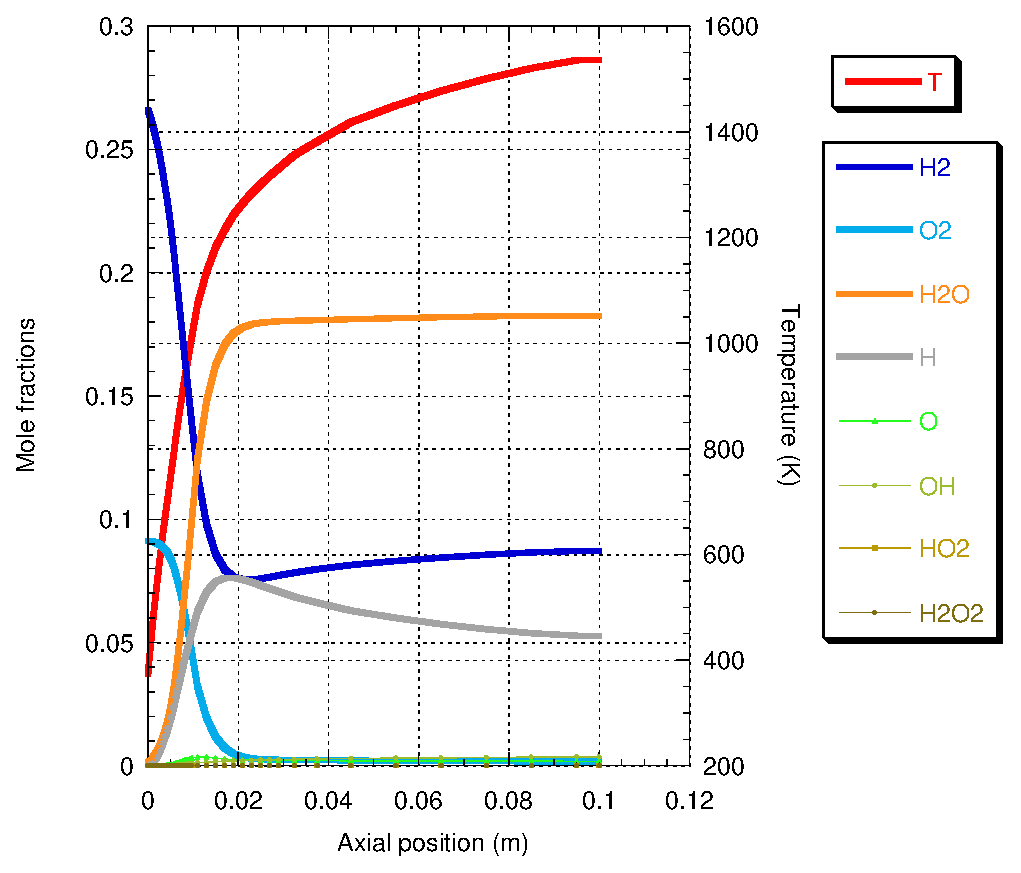
\includegraphics[scale=0.7]{premix_profile.eps}
\caption{Species profiles and temperature profile for hydrogen oxidation mechanism}
\end{figure*}


%===============================================================================================
%
%
%
%===============================================================================================

